%# -*- coding:utf-8 -*-
\section{Methodologies}
\label{sec3_3}

In this section the overall processing pipeline is discussed and the techniques used for the lumen segmentation of the abdominal aorta from CTA are detailed.
% The original data adopted in our work is a series of CTA images with the dimension of $512\times512\times90$.
% The series are acquired from the trunk of the patient with CVDs.

The overall design of the pipeline is illustrated in Fig. \ref{fig:DataFlow}.
The format and data type of original images are firstly converted.
Then the conditioned data is fed into two branches to produce the two inputs required by the main segmentation module.
One branch performs several preprocessing work on the images to produce the feature images. %, including smoothing, gradient magnitude computation, and intensity mapping.
And the other branch computes the initial level sets of the images. %, including a mini level set branch which requires numbers of seeds.
After the branches end the computation, their production are fed into the main segmentation module, where the actual interface evolution takes place.
In the final phase, the output level sets are extracted and then visualized by using a surface rendering technique.
%The parameters and seeds are provided manually and tuned repeatedly during the processing.
\begin{figure}[t]
\centering
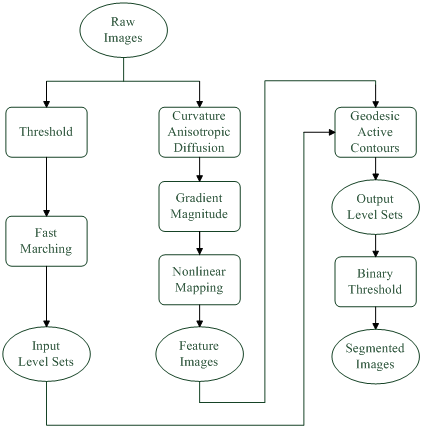
\includegraphics[width=3.2in]{Figures/chap03/DataFlow.png}
\caption{An overview of the segmentation pipeline.}
\label{fig:DataFlow}
\end{figure}

\subsection{Preprocessing}

Before the main processing begins, several necessary pretreatment on the original images should be done.
By considering the requirements of the methods chosen for this job, the preprocessing should include the production of feature images, and the generation of input level sets.
The feature images provide the main level set method with the ``maps" about where to stop, while the input level sets give the main functioning module the initial contours from where the actual interface evolution begins.

\subsubsection{Production of Feature Images}

%The branch of feature image production is depicted in Fig. \ref{fig:DataFlow}.
Image smoothing is a necessary job due to the original series acquired from the medical modality are often mixed with some noisy pixels.
What to take care of is that the original edges of the target (i.e., aorta) should be preserved as completely as possible while removing the noises.
Bear this in mind, a level-set curvature method with variable conductance \cite{Whitaker2001} is chosen for the job.
This method is good at enhancing and preserving edges, and is robust to the edge contrast.
It can be described as the following \emph{modified curvature diffusion equation} (MCDE):
\begin{equation}
\label{eqn:MCDE}
I_t = |\nabla I| \nabla \cdot c(|\nabla I|) \frac{\nabla I}{|\nabla I|},
\end{equation}
where $I = I(x, y, 0)$ represents the input image, $I_t(\cdot) = I(x, y, t)$ represents the output image generated over time $t$, and $c$ is the conductance function given by
$c(|\nabla I|) = k^2/(k^2 + |\nabla I|^2)$ with $k$ a parameter which determines the contrast of boundaries that will have significant effects on the smoothing.

After that, the computation of gradient magnitude is performed on the resulting series to detect the edge of target.
Since the feature images to be produced are required by the downstream geodesic active contours module, the most important step in this series of tasks is the computation of the magnitude of gradient pixel-wisely for the images:
\begin{equation}
\label{eqn:Gaussian}
I_{grad} = \exp(-|(\nabla \ast G) \cdot I_t|),
\end{equation}
where $I_{grad}$ is magnitude of the gradient at some point in the image, and $\nabla \ast G$ means the first order derivative of a Gaussian operator.

The computed edge images are mapped through a nonlinear relation (usually represented in the form of an S-shaped function) in order to get the feature images:
\begin{equation}
\label{eqn:Sigmoid}
I_{\sigma} = (I_{max} - I_{min}) \cdot \frac{1}{1 + \exp\left(-\frac{I_{grad} - n}{m}\right)} + I_{min},
\end{equation}
where $I_{\sigma}$ denotes the intensity values of the output image, $I_{max}$ and $I_{min}$ represent the maximum and minimum of the output intensity values, respectively; $m$ is a constant that controls the width of the input intensity range, and $n$ is a constant that gives an intensity around which the range is centered.
The mapping results may vary due to different choices of the parameters for the individual modules in the pipeline.

\subsubsection{Semi-Automatic Generation of Input Level Sets}

%The initial level set generation branch is parallel to the above one, which is responsible for the computation of the values required by the main evolution as its input level sets (see Fig. \ref{fig:DataFlow}).
% This branch is a mini level set that takes numbers of seeding points (or seeds) before the computation begins.
The first pass is a thresholding procedure that will strip out most of the irrelevant details of the images.
After the thresholding is done, the fast marching algorithm \cite{Sethian1999} could focus its evolution on the target with the appropriately selected seeding points.
For the curve $\mathcal{C}$ evolving over time $t$
\begin{equation}
\label{eqn:Curves}
\mathcal{C}(t) = \{(x,y) | T(x,y) = t\},
\end{equation}
where $(x,y)$ represents some point in the image, and $T(x,y)$ is the time of arrival.
The algorithm solves the following Eikonal equation (which is in fact a stationary Hamilton-Jacobi equation)
\begin{equation}
1 = | \nabla T | F,
\end{equation}
where $F$ denotes the velocity in the normal direction at some point $(x,y)$.
$\mathcal{C}$ propagates inwards when $F < 0$; it propagates outwards when $F > 0$.
The results of this computation are the time-crossing map in which contains of a series of curve interfaces at different time of evolution.

\subsection{Geodesic Active Contours Evolution}

%The module that actually working towards the segmentation is illustrated in Fig. \ref{fig:DataFlow}.
At this point, the geodesic active contours module has its two inputs available: the feature images and the initial level sets.
The feature images provide the maps for the interface evolution initialized by the input level sets.
The classical ``snakes" or active contour models for boundary detection were proposed by Kass et al. \cite{Kass1988}.
The idea is to evolve a contour $\mathcal{C}$ such that the edge of the object can be detected.
This evolution is achieved by minimizing an energy functional whose (local) minimum can be found at the edge of the object.
% This energy functional of the contour $\mathcal{C}_0$ in the classical snakes approach is given by (the denotation is adopted from \cite{Caselles1997})
% \setlength{\arraycolsep}{0.0em}
% \begin{eqnarray}
% \label{eqn:Snakes}
% E(\mathcal{C})&{}={}&\alpha \int_0^1 |\mathcal{C}'(q)|^2 dq + \beta \int_0^1 |\mathcal{C}''(q)|^2 dq \nonumber \\
                  % &&{-}\:\lambda \int_0^1 |\nabla I ( \mathcal{C}(q) ) | dq,
% \end{eqnarray}
\setlength{\arraycolsep}{5pt}
% where $\mathcal{C}(q)$ denotes the parametrized planar curve $\mathcal{C}(q):[0,1]\rightarrow \mathrm{R}^2$, $I:[0,a]\times [0,b]\rightarrow \mathrm{R}^{+}$ represents an image on which the edge detection task is carried out, and $\alpha$, $\beta$, and $\lambda$ are all real positive constants.
% The first two components control the smoothness of the curves to be detected, and the last one propagates the curve outwards (or inwards) until it ``touches" boundaries of the objects in the given image.
% The classical problem is to find the curve $\mathcal{C}$ that minimizes the energy functional $E$, for the given constants $\alpha$, $\beta$, and $\lambda$.
However, the curve in this approach cannot deal with the change of its topology so that detecting more than one object in the image is impossible without additional procedures \cite{Caselles1997}.
Caselles \textit{et al.} \cite{Caselles1997} improved the classical ``snakes" by proposing the geodesic active contours method, which allows to detect both the internal and external boundaries of several objects simultaneously.
This method incorporates the concepts of geodesic computation and level set evolution.
The proposed model is a particular case of the classical model:
\begin{equation}
\label{eqn:ParticularSnakes}
E(\mathcal{C}) = \alpha \int_0^1 | \mathcal{C}'(q) |^2 dq - \lambda \int_0^1 | \nabla I_{s} ( \mathcal{C}(q) ) |dq,
\end{equation}
where $\mathcal{C}(\cdot)$ denotes the parametrized planar curve $\mathcal{C}(q):[0,1]\rightarrow \mathrm{R}^2$, $I_{s}:[0,a]\times [0,b]\rightarrow \mathrm{R}^{+}$ represents an image on which the edge detection task is carried out.

To minimize the functional defined by (\ref{eqn:ParticularSnakes}), the curve at the points of maxima $|\nabla I_{s}|$ must be located.
During this process, certain level of smoothness of the curve also needs to be kept.
In (\ref{eqn:ParticularSnakes}), $|\nabla I_{s}|$ can be substituted by $-g(|\nabla I_{s}|)$, where $g(\cdot): [0, \infty) \rightarrow \mathrm{R}^{+}$ is a monotonically decreasing function. %such that $\lim_{x \to \infty} g(x) = 0}$.
Hence, a general energy functional is obtained
\begin{equation}
\label{eqn:GeneralEnergy}
E(\mathcal{C}) = \alpha \int_0^1 | \mathcal{C}'(q) |^2 dq + \lambda \int_0^1 g( | \nabla I_{s} ( \mathcal{C}(q) ) | )^2 dq.
\end{equation}
The aim of the evolution is trying to obtain
\begin{equation}
\label{eqn:MinModel}
\min \int_0^1 g(|\nabla I_{s} ( \mathcal{C} (q) )|) |\mathcal{C}' (q)| dq.
\end{equation}
% Thus the problem has been shifted from the minimization of (\ref{eqn:ParticularSnakes}) to the geodesic computation.
In (\ref{eqn:GeneralEnergy}), $g(\cdot)$ is equivalent to the speed of the evolution of the curve.
And it is also dependent upon the geometry of the image content.
For the ideal edges of the objects to be detected, the choice of parameter $g(\cdot)$ is independent of their geodesic computation.
So the minimum given in (\ref{eqn:MinModel}) can be rewritten as:
\begin{equation}
\label{eqn:MinModel2}
\min \int_0^1 g(I_{\sigma}) |\mathcal{C}' (q)| dq.
\end{equation}
To obtain the minimum given in (\ref{eqn:MinModel2}), the following Euler-Lagrange associated with this model needs to be calculated
\begin{equation}
\label{eqn:EvolutionModel}
\frac{\partial \mathcal{C}(t)}{\partial t} = g(I_{\sigma}) \kappa \mathcal{N} - (\nabla g(I_{\sigma}) \cdot \mathcal{N}) \mathcal{N},
\end{equation}
where $\kappa$ is the curvature of $\mathcal{C}(t)$, $\mathcal{N}$ is the unit inward normal vector. %, and the right-hand side of the equation is the computation of Euler-Lagrange.
This equation presents the way $\mathcal{C}$ evolving towards the boundaries of the objects to be detected.
The initial curve is marked as $\mathcal{C}(0) = \mathcal{C}_0$, which evolves to a (local) minimum of (\ref{eqn:MinModel2}).

According to (\ref{eqn:EvolutionModel}), this evolution will stop when $\frac{\partial \mathcal{C}(t)}{\partial t} = 0$, meaning that the boundaries of the objects are detected.
Suppose that the curve $\mathcal{C}$ is a level-set of a function $u(\cdot):[0,a] \times [0,b] \rightarrow \mathrm{R}$.
Regarding (\ref{eqn:MinModel2}) and (\ref{eqn:EvolutionModel}), the former geodesic calculation is transformed to finding the steady state solution of the following equation:
\begin{equation}
\label{eqn:LevelSetModel}
\begin{split}
\frac{\partial u}{\partial t} & = |\nabla u| \textrm{div} \left(g(I_{\sigma}) \frac{\nabla u}{|\nabla u|}\right) \\
                              %& = g(I_{\sigma}) |\nabla u| \textrm{div} \left(\frac{\nabla u}{|\nabla u|}\right) + \nabla g(I_{\sigma}) \cdot \nabla u \\
                              & = g(I_{\sigma}) |\nabla u| \kappa + \nabla g(I_{\sigma}) \cdot \nabla u,
\end{split}
\end{equation}
where $\kappa = \textrm{div}\left(\frac{\nabla u}{|\nabla u|}\right)$.
The right-hand side of this equation is the Euler-Lagrange of (\ref{eqn:MinModel2}).
% Here in this equation, $u$ is the embedding function mentioned above that deforms according to $u_t = \beta |\nabla u|$, where $\beta$ is a function computed on the level sets.
% From the perspective of image segmentation, a positive real constant $c$ is introduced in order to detect the boundaries of a non-convex object using a convex initial curve
% \begin{equation}
% \label{eqn:ImprovedLevelSetModel}
% \begin{split}
% \frac{\partial u}{\partial t} & = g(I) |\nabla u| \textrm{div} \left(\frac{\nabla u}{|\nabla u|}\right) + c g(I) |\nabla u| \\
                              % & = g(I) ( \kappa + c ) |\nabla u|.
% \end{split}
% \end{equation}

In order to increase the ``attractive force" to the contour towards the edges and allow the detection of non-convex objects, the term $cg(I_{\sigma})|\nabla u|$ is added to (\ref{eqn:LevelSetModel}):
\begin{equation}
\label{eqn:Geodesic1}
\frac{\partial u}{\partial t} = |\nabla u| \textrm{div} \left(g(I_{\sigma}) \frac{\nabla u}{|\nabla u|}\right) + c g(I_{\sigma}) |\nabla u|,
\end{equation}
where $c$ is a constant and $c \in \mathrm{R}^+$.
Regarding (\ref{eqn:LevelSetModel}), the above equation can be rewritten as
\begin{equation}
\label{eqn:Geodesic2}
\frac{\partial u}{\partial t} = g( I_{\sigma} )( c + \kappa ) |\nabla u| + \nabla u \cdot \nabla g(I_{\sigma}).
\end{equation}
% which means that the level sets move according to
The above equation can be transformed to the following equation
\begin{equation}
\label{eqn:Geodesic3}
\frac{\partial \mathcal{C}}{\partial t} = g(I_{\sigma}) ( c + \kappa ) \mathcal{N} - ( \nabla g(I_{\sigma}) \cdot \mathcal{N} ) \mathcal{N}.
\end{equation}
The solution to this object detection problem is equivalent to the zero level-set of the steady state ($u_t = 0$) of (\ref{eqn:Geodesic1}).
%Comparing (\ref{eqn:EvolutionModel}) and (\ref{eqn:Geodesic3}), one can find an added term $c g(I_{\sigma}) \mathcal{N}$, which is corresponding to the
% For the ideal edges of the objects to be detected, the choice of parameter $g$ is independent of their geodesic computation.
% It is a very simple edge detector which is given by the following equation
% \begin{equation}
% \label{eqn:EdgeDetector}
% g = \frac{1}{1+\|\nabla \hat{I}\|^p},
% \end{equation}
% where $\hat{I}$ denotes a Gaussian-smoothed image of the original $I$ and $p$ is the exponential of $\hat{I}$.
% What we are interested in is the time when the curve interface corresponding to the edges of the target.
% After the evolution stopped, a binary thresholder is provoked to take a ``snapshot" of this interface.
% This resulting level set should be the edges of the objects to be detected.

\subsection{Surface Extraction}

To visualize the surface model, the surface information should be firstly extracted by the marching cubes method \cite{Lorensen1987MC}.
As the initial step of surface extraction, arrays of cubes are created from the input with each cube consisting of eight pixels (four from one slice and the other four from the next slice).
Then the index for each cube is calculated by comparing the eight intensity values to the specified isovalue corresponding to the surfaces of the objects.
By referring to the triangulated cases with the indexes, the intersection patterns of the objects and the cubes can be roughly determined.
Then the precise edge intersections are computed using linear interpolation with the intensity values at each vertex of the cubes.
After that, the unit normals to the surface at each vertex of these cubes are computed via central differences.
The resulting triangles are then sent to the graphics systems and displayed by standard rendering techniques.
% The isovalue representing the edge of the segmented target is selected.
% Then the 3-D model of the target can be reconstructed.
% That is the 3-D surface model of the lumen of the aorta.